\documentclass[12p]{article}
\usepackage[utf8]{inputenc}
\usepackage[english]{babel}

\usepackage{graphicx}
\usepackage{hyperref}
\usepackage{caption}
\usepackage{mathtools}
\usepackage{lscape}
\usepackage{numprint}

\usepackage[backend=biber,style=iso-numeric,sorting=none]{biblatex}
\bibliography{references.bib}

\title{Exoplanet Ranking \\\large Introduction to Data Science}
\date{\today}
\author{
    Goron, Nathan \\ \texttt{\href{mailto:nathan.goron@helsinki.fi}{nathan.goron@helsinki.fi}}
    \and 
    Motzkus, Franz \\ \texttt{\href{mailto:franz.motzkus@helsinki.fi}{franz.motzkus@helsinki}}
    \and 
    Vopat, Tomáš  \\ \texttt{\href{mailto:tomas.vopat@helsinki.fi}{tomas.vopat@helsinki.fi}}
}

%------------------------------------------------------------------
%------------------------------------------------------------------

\begin{document}

\maketitle

\section{Introduction}

As mankind faces environmental problems nowadays, several approaches come up with the solutions. One way is to modify our habits to act softly with nature, the other way is to find another place to new inception.

In this project, we aim to find an appropriate exoplanet (a planet in another solar system) that might be good enough for life. To deal with this issue, we use data about known exoplanets and AI techniques. The domain of this attempt is to provide an answer whether there is the planet in the universe similar to the Earth or not. To achieve the goal we compute the similarity rank for each exoplanet.

This study might interest companies, that want to raise people's curiosity around the topic of finding Earth-like planets, or simply astronomy enthusiast, that we can inspire with a new view.

%------------------------------------------------------------------

\section{Preprocessing and Analysis}
The dataset~\cite{dataset} we used is from an archive hosted by the NASA exoplanet science institute which is operated by the California Institute of Technology. In the dataset, there is data about \numprint{4056} exoplanets with \numprint{47} various attributes (e.g.\ temperature, star luminosity, distance). These attributes are used to determine the ``livability score'' since they influence if humanity could survive on this planet.

As a first step, we removed the columns, that contained irrelevant information for our goals such as website links or different names of the exoplanet. Next step was to drop columns with a high ration of missing data. In the column \verb|fpl_eccen| is \numprint[\%]{61.7} missing and in the column \verb|fst_spt| \numprint[\%]{66.3}. As a result only \numprint{20} columns left for the ranking, these attributes are deeply described in Figure~\ref{tab:att_desc}. Since the domain knowledge of physicists, astrologists and maybe even biologists are needed, we use all the attributes mentioned above for our experiments. For further experiments, it is supposed to consult with a specialist the livability impact of each attribute in the dataset, as some of those might be more important than the others.

Afterwards, we explored the distributions of each variable. As some of the variables vary a lot, some of them are almost constant across all the dataset. To make it more clear, we plot the mean value of each variable with its standard deviation in Figure~\ref{pic:mean}. As can be seen, attributes like \verb|fst_mass| (stellar mass) or \verb|fst_lum| (stellar luminosity) have small in comparison to others. On the other hand, \verb|fst_teff| (effective temperature) and \verb|fpl_orbper| (orbit period) differ a lot. To be able to plot all the variables, it was necessary to log-scale all the values. 

Furthermore, some of the variables might be correlated (mutually influenced). Due to that, we have computed correlation matrix for each pair of variables. As illustrated by Figure~\ref{pic:corr}, \verb|fst_logg| (gravity acceleration at the stellar surface) and \verb|fst_lum| (stellar luminosity) are highly correlated, which means that with the gravity acceleration the luminosity of the star decreases.

To finish the analysis, we try to group exoplanets by its properties, as the planets are situated in the vector space (not in the universe). First of all, we have to normalize all the values to be in the same range (from 0 to 1). After that, the clustering can be applied. We use the K-Means algorithm implemented in \textit{Scikit-learn}\footnote{\url{https://scikit-learn.org}} library for machine learning. Surprisingly, the optimal number of clusters is \numprint{2}, since there are \numprint{4} thousand exoplanets in the dataset.

We can see in Figure~\ref{pic:cluster} that the Earth is situated in the green cluster where is \numprint[\%]{77.5} of the exoplanets. The planets are distinguishable even though space is projected by Singular-Value Decomposition (SVD, \textit{Scikit-learn}\footnotemark[\value{footnote}] implementation is used) into 2 dimensions.

\begin{figure}\centering
    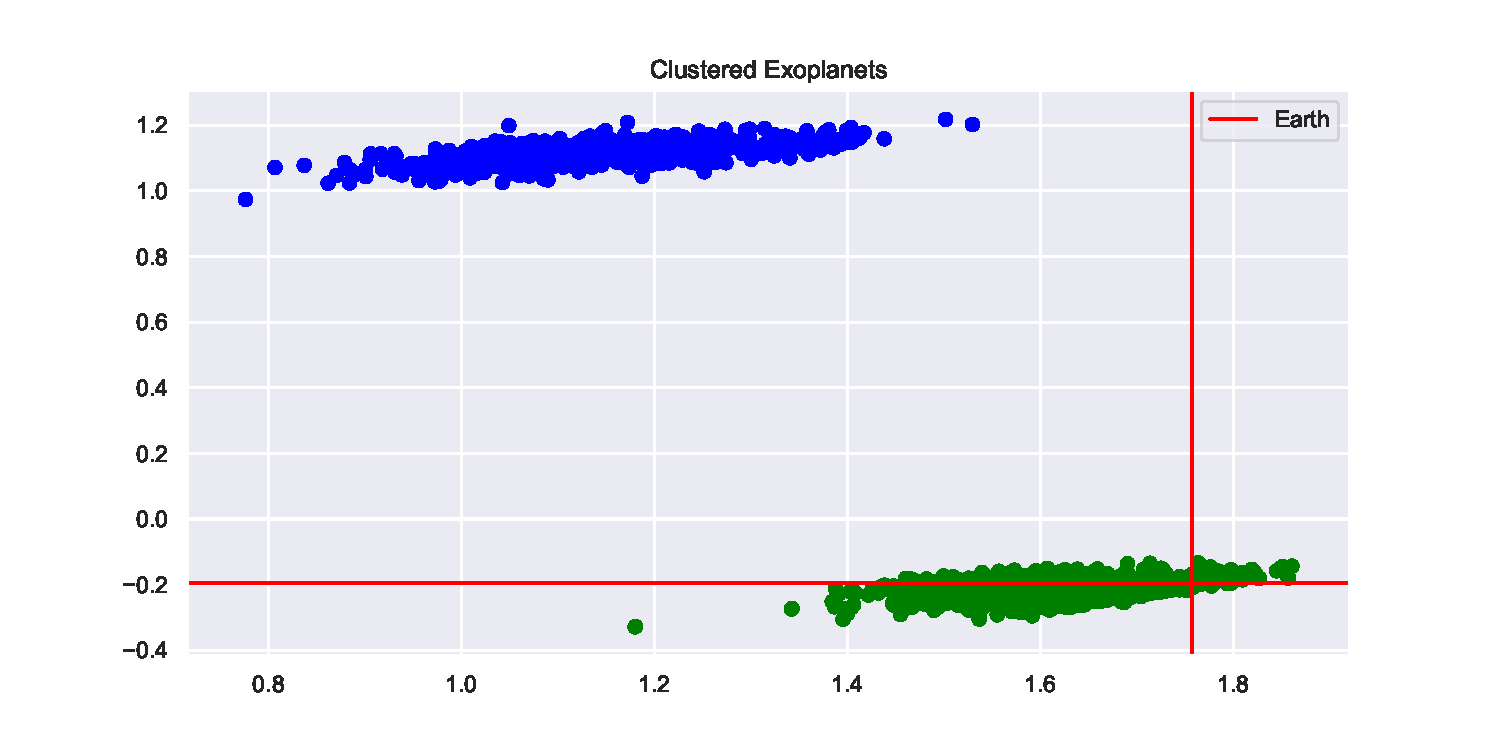
\includegraphics[width=0.9\textwidth]{graphics/cluster.pdf}
    \caption{K-Means Clustering the Exoplanets projected by SVD into 2 dimensions}
    \label{pic:cluster}
\end{figure}

%------------------------------------------------------------------

\section{Exoplanet Ranking}
To compute the ranking we use vector similarity between each exoplanet and the Earth. All those vectors are obtained from the Exoplanet dataset. The vectors are preprocessed, so there is not any missing data and the values are normalized. The ranking output is a value for each exoplanet in the range from 0 to 10 (rescaled by multiplying) where 10 means the most similar planet.

Cosine distance implemented in \textit{Scikit-learn}\footnotemark[\value{footnote}] library is used as a similarity measure between vectors. The presumption is that the most similar exoplanets to the Earth are the most likely sufficient for life. The exact formula is displayed in Formula~\ref{eq:cosine}.

\begin{align}
    \text{cosine}(u,v) &= \frac{\sum_{i=0}^{n-1} u_iv_i  }{ \sqrt{\sum_{i=0}^{n-1} u_i^2  } \sqrt{\sum_{i=0}^{n-1} v_i^2  }} \label{eq:cosine}
\end{align}

It is supposed that some parameters have a bigger impact than others on how ``livable`` an exoplanet is. For instance, the metal abundance is probably not as important as surface temperature. Therefore two rankings have been computed -- the second one takes into account the weight of the parameters.

We created a weight vector $w$ that can be seen in Table~\ref{tab:att_desc} with weight in the range from 1--10 for each attribute of exoplanets. To compute the weighted cosine similarity the library \textit{SciPy}\footnote{\url{https://www.scipy.org}} is used. Where it is implemented as a correlation between vectors with weighted averages as describe Formula~\ref{eq:cosine_weighted} and Formula~\ref{eq:weighted_mean}, where $u$ and $v$ are the vectors of exoplanets.

\begin{align}
\text{cosine}_{\text{weighted}}(u,v,w) &= \frac{\sum_{i=0}^{n-1} (u_i-\overline{u_w})(v_i-\overline{v_w})  }{ \sqrt{\sum_{i=0}^{n-1} (u_i-\overline{u_w})^2  } \sqrt{\sum_{i=0}^{n-1} (v_i-\overline{v_w})^2  }} \label{eq:cosine_weighted} \\
\overline{u_w} &= \frac{ \sum_{i=0}^{n-1} u_iw_i }{ \sum_{i=0}^{n-1} w_i } \label{eq:weighted_mean}
\end{align}

%------------------------------------------------------------------

\section{Web App}
For our product, we created a Node.js\footnote{\url{https://nodejs.org}} web application to display the results of our ranking. The website uses native HTML/CSS/JS with Bootstrap\footnote{\url{https://getbootstrap.com}} classes, a node.js template engine called EJS\footnote{\url{https://ejs.co}} to pass data to views as well as some data visualisation frameworks such as chart.js to make it easier to display our data.

The Web App displays the ranking, so the user can directly compare both variants of the ranking (the standard and the weighted one). Underneath there is a bar chart showing the number of exoplanets discovered in each year from 1991 to 2019, where a remarkable amount of exoplanets was discovered in years 2014 and 2016. In the end, the distance of the top \numprint{20} planets is displayed. All the plots and the tables react to the user's mouse hover to show more details about the specific object.

Design is meant to be a little mysterious to catch the eye of potentially interested people since the website is meant to be presented on fairs or other events. The homepage shows features like the caption and an image of a planet on the colourfully modified background to be quickly recognized by astronomy enthusiasts and other people enjoying the wonders of outer space.

Currently, the website can be reached at \url{http://ec2-52-201-232-146.compute-1.amazonaws.com:3000}.

%------------------------------------------------------------------

\section{Results}
According to our ranking, the most suitable exoplanet is \verb|K2-85 b| with a score of \numprint{9.96} for the regular ranking and \numprint{9.94} for the weighted ranking. The temperature of \numprint[K]{351}, which is a lot for a human to withstand without proper equipment, but looking at the repartition of the temperature column in the dataset, this is a pretty good result. We can also note that the density is very similar to Earth's, and therefore the gravity wouldn't make feel much different for a human.

On the other hand, the worst planet for the weighted ranking is \verb|BD+20 2457 b|, with a score of \numprint{4.21} out of \numprint{10}. In addition to being \numprint[pc]{4762} away from Earth (it would take \numprint{13821} years travelling at the speed of light to reach it), it's surface temperature is about \numprint[K]{2370}, which makes it a really bad choice to be mankind's next home.

Even though providing a reliable ranking would require a deeper knowledge of astronomy, we can safely (but naively) say that our ranking gives a good glimpse of what could be mankind's next home.

%------------------------------------------------------------------

\printbibliography

\appendix
\begin{landscape}
    \section{Dataset Attributes}
    \begin{table}[!h]\centering
        \caption{Attributes Description}
        \label{tab:att_desc}
        \begin{tabular}{|l l c c |}\hline
            Attribute         & Description                                         & Unit          & Weight \\ \hline\hline
            fpl\_orbper      & orbital period                                     & days            & 5 \\ \hline
            fpl\_smax        & the longest radius of an elliptic orbit    & AU             &3 \\ \hline
            fpl\_bmasse    & mass of the planet                              & Earth mass & 5 \\ \hline
            fpl\_rade         & planet radius                                       & Earth radii    & 5 \\ \hline
            fpl\_dens        & density of the planet                            & $g/cm^3$  & 7 \\ \hline
            fpl\_tranflag    & wether the lanet transits the star or not & bool          & 1 \\ \hline
            fpl\_cbflag      & does planet orbit a binary solar system  & bool           & 5 \\ \hline
            fpl\_snum       & number of stars in the solar system      & integer        & 8 \\ \hline
            dec                 & declination of the planetary system       & decimal degrees & 3 \\ \hline
            fst\_teff          & effective temperature                          & K                 & 10 \\ \hline
            fst\_logg        & gravity acceleration at the star surface  & $\log_{10}{\left( \text{cm}/s^2\right)}$ & 4 \\ \hline
            fst\_lum         & star lumonisty                                     & $\log_{10}{\left( \textit{Solar luminosty}\right)}$ & 4 \\ \hline
            fst\_mass       & stellar mass                                        & Solar mass  & 6 \\ \hline
            fst\_rad         & stellar raidus                                        & Solar radii    & 6 \\ \hline
            fst\_met        & star metallicity                                      & dex            & 3 \\ \hline
            fst\_metratio & metal abundance                                    & [Fe/H], [M/H]  & 1 \\ \hline
            fst\_age         & stellar age                                            & Gyr              & 8 \\ \hline
        \end{tabular}
    \end{table}
    
    \newpage
    \section{Charts}
    \begin{figure}[!ht]\centering
        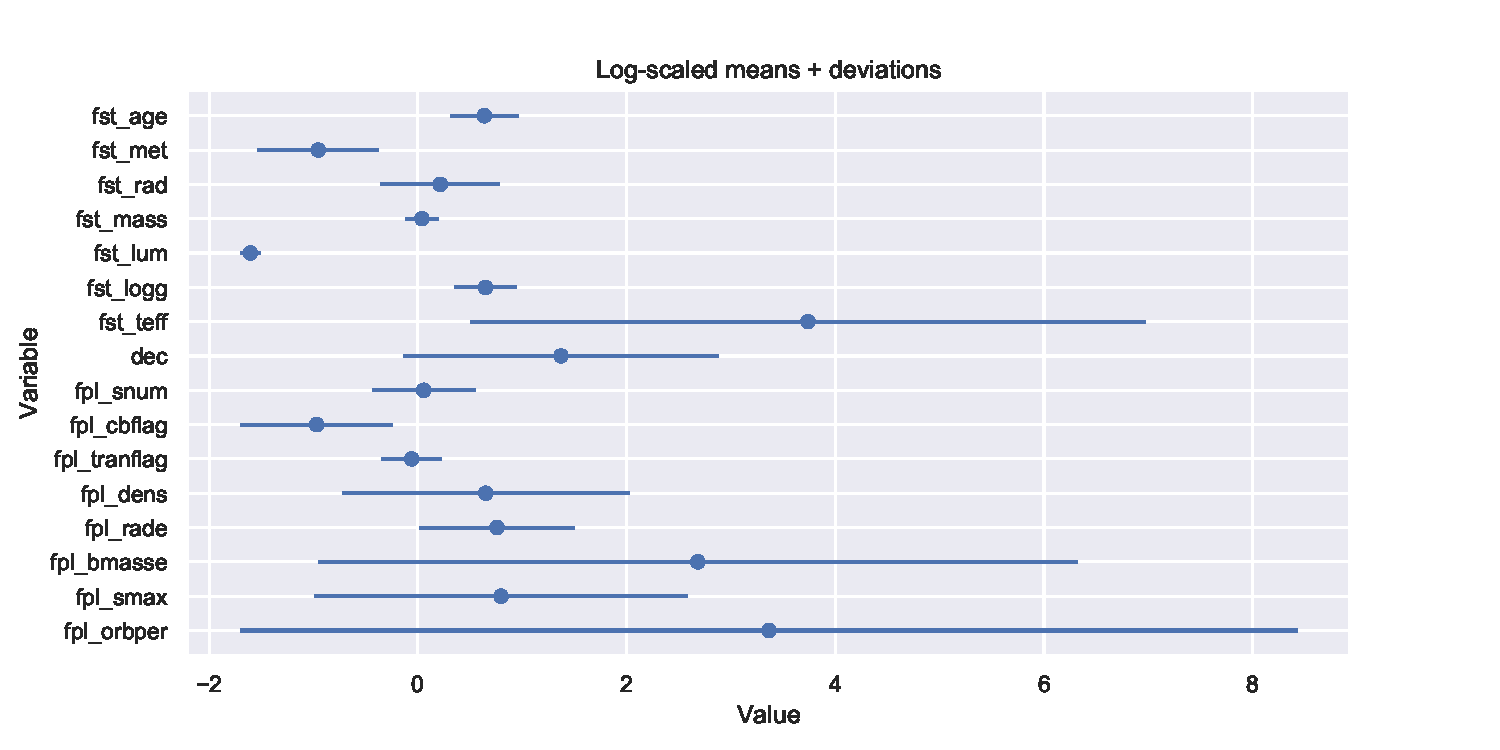
\includegraphics[width=1.5\textwidth]{graphics/mean_deviation.pdf}
        \caption{log-scaled mean of each variable with its standard deviation}
        \label{pic:mean}
    \end{figure}
    
    \begin{figure}[!ht]\centering
        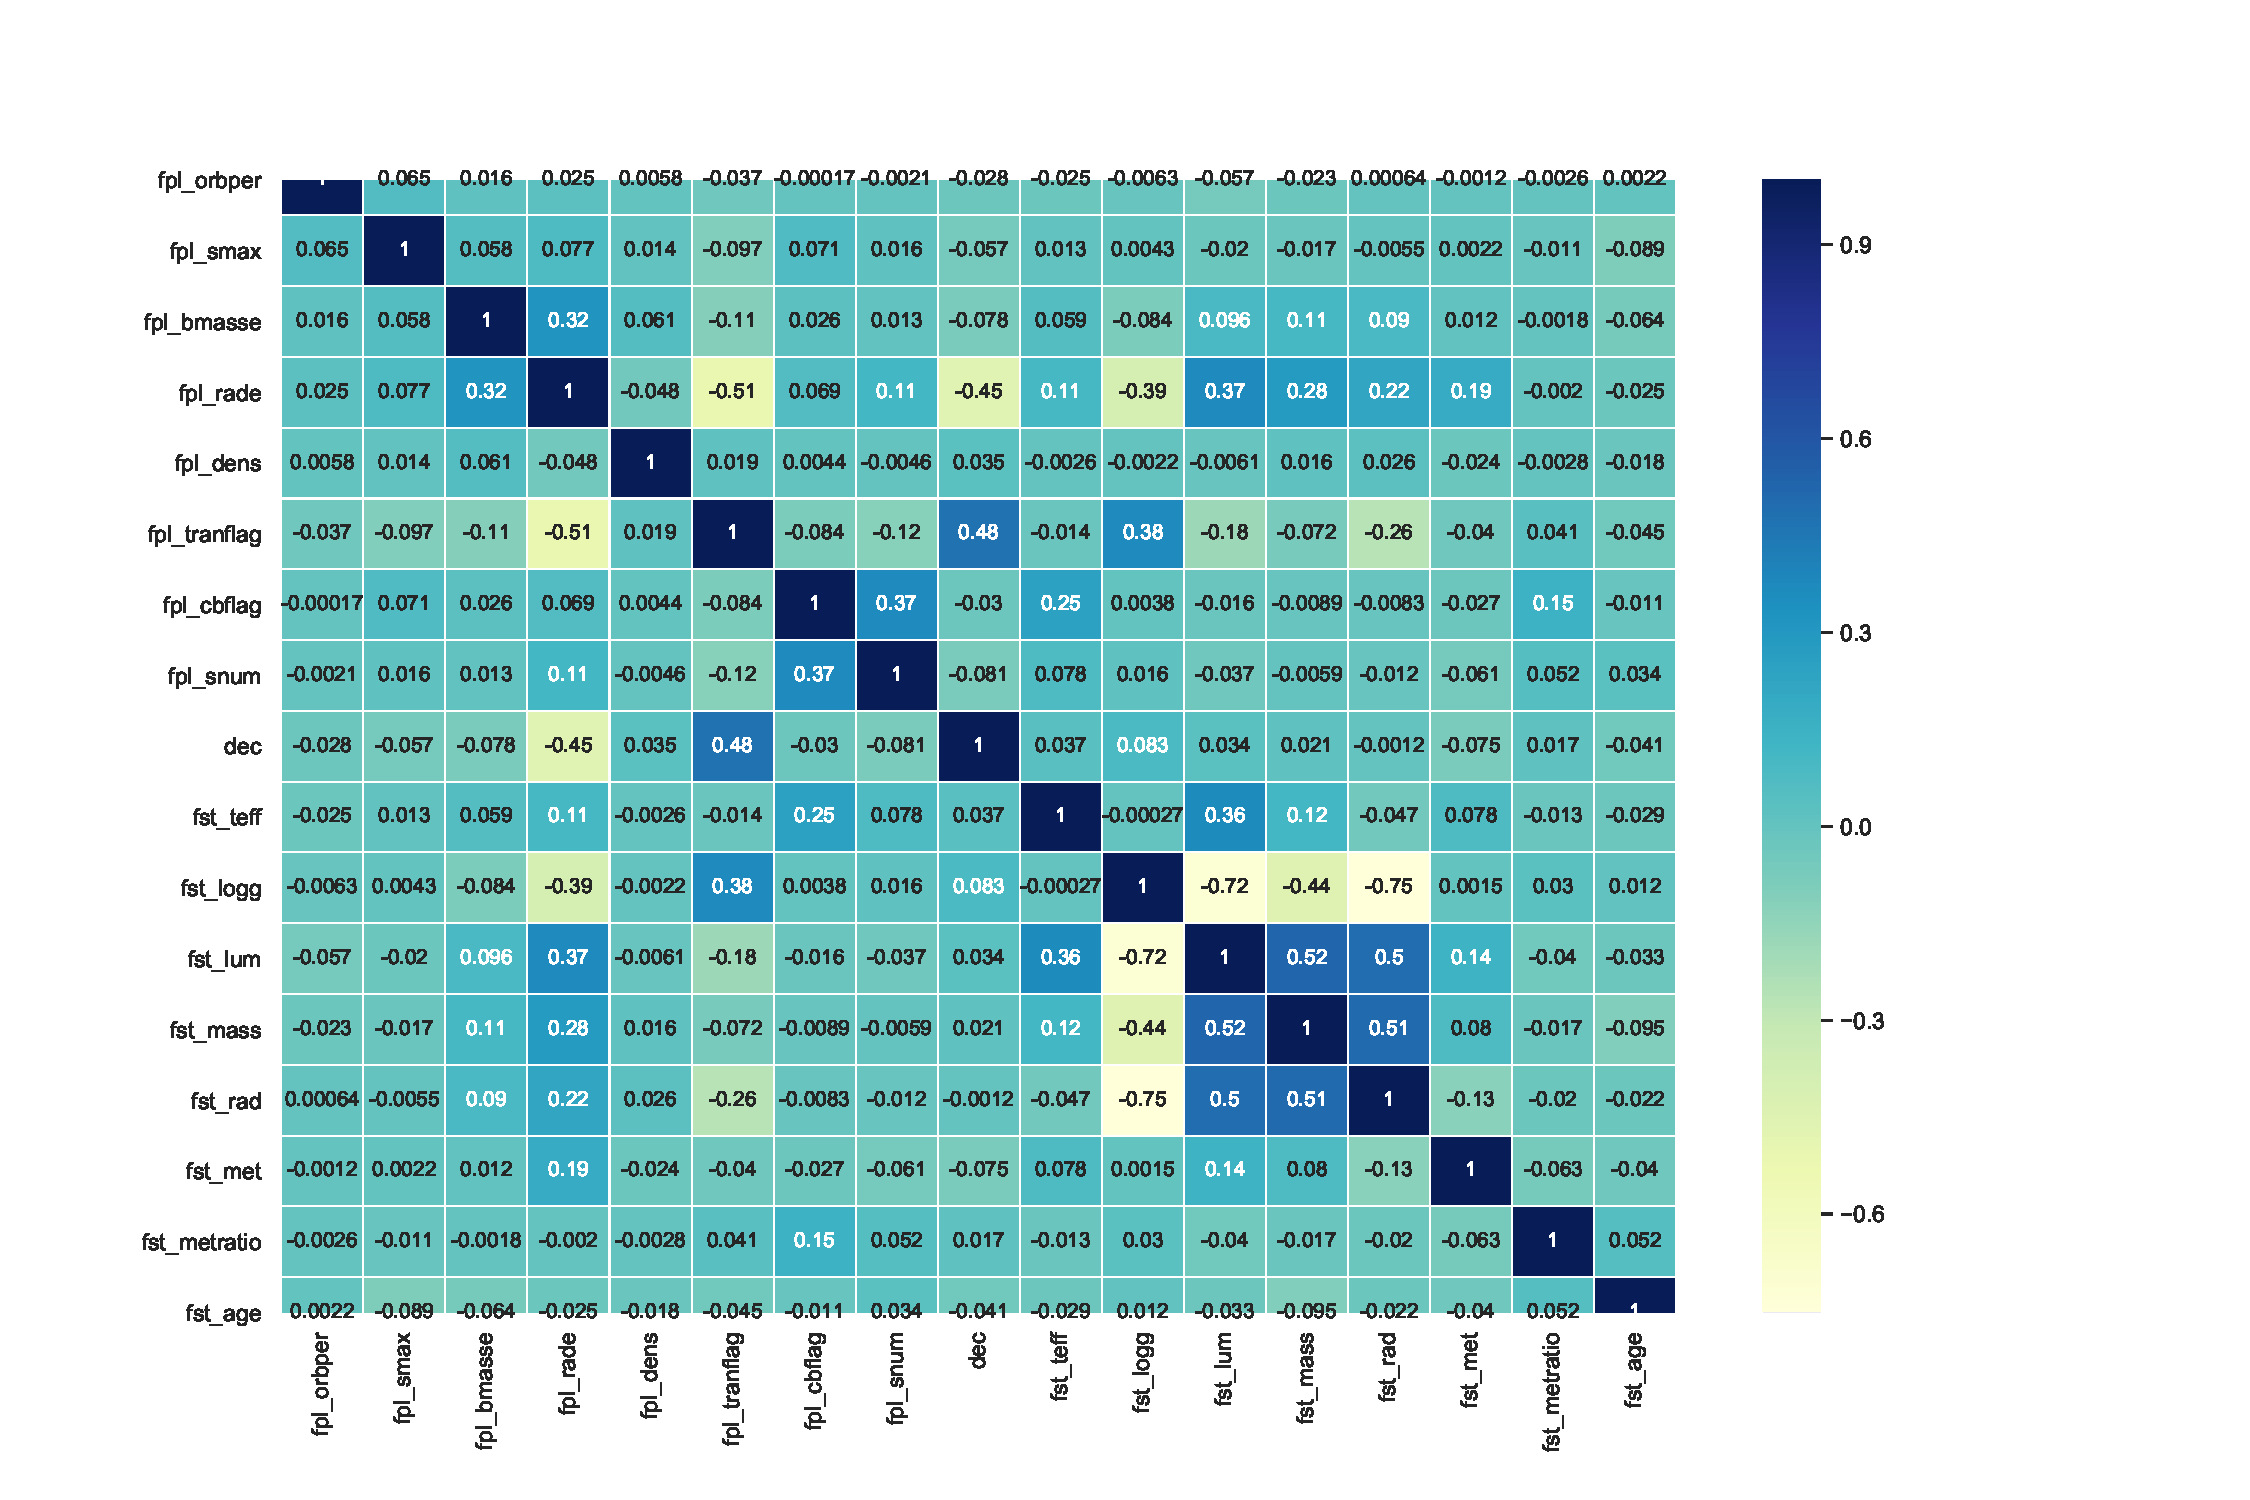
\includegraphics[width=1.8\textwidth]{graphics/correlation_matrix.pdf}
        \caption{correlation matrix of variables}
        \label{pic:corr}
    \end{figure}
\end{landscape}

\end{document}
